%%% Template originaly created by Karol Kozioł (mail@karol-koziol.net) and modified for ShareLaTeX use

\documentclass[a4paper,11pt]{article}

\usepackage[T1]{fontenc}
\usepackage[utf8]{inputenc}
\usepackage{graphicx}
\usepackage{xcolor}

\renewcommand\familydefault{\sfdefault}
\usepackage{tgheros}
\usepackage[defaultmono]{droidmono}

\usepackage{amsmath,amssymb,amsthm,textcomp}
\usepackage{enumerate}
\usepackage{multicol}
\usepackage{tikz}

\usepackage{geometry}
\geometry{total={210mm,297mm},
left=25mm,right=25mm,%
bindingoffset=0mm, top=20mm,bottom=20mm}


\linespread{1.3}

\newcommand{\linia}{\rule{\linewidth}{0.5pt}}

% custom theorems if needed
\newtheoremstyle{mytheor}
    {1ex}{1ex}{\normalfont}{0pt}{\scshape}{.}{1ex}
    {{\thmname{#1 }}{\thmnumber{#2}}{\thmnote{ (#3)}}}

\theoremstyle{mytheor}
\newtheorem{defi}{Definition}

% my own titles
\makeatletter
\renewcommand{\maketitle}{
\begin{center}
\vspace{2ex}
{\huge \textsc{\@title}}
\vspace{1ex}
\\
\linia\\
\@author \hfill \@date
\vspace{4ex}
\end{center}
}
\makeatother
%%%

% custom footers and headers
\usepackage{fancyhdr}
\pagestyle{fancy}
\lhead{}
\chead{}
\rhead{}
\lfoot{Assignment : 1}
\cfoot{}
\rfoot{Page \thepage}
\renewcommand{\headrulewidth}{0pt}
\renewcommand{\footrulewidth}{0pt}
%

% code listing settings
\usepackage{listings}
\lstset{
    language=Python,
    basicstyle=\ttfamily\small,
    aboveskip={1.0\baselineskip},
    belowskip={1.0\baselineskip},
    columns=fixed,
    extendedchars=true,
    breaklines=true,
    tabsize=4,
    prebreak=\raisebox{0ex}[0ex][0ex]{\ensuremath{\hookleftarrow}},
    frame=lines,
    showtabs=false,
    showspaces=false,
    showstringspaces=false,
    keywordstyle=\color[rgb]{0.627,0.126,0.941},
    commentstyle=\color[rgb]{0.133,0.545,0.133},
    stringstyle=\color[rgb]{01,0,0},
    numbers=left,
    numberstyle=\small,
    stepnumber=1,
    numbersep=10pt,
    captionpos=t,
    escapeinside={\%*}{*)}
}

%%%----------%%%----------%%%----------%%%----------%%%

\begin{document}

\title{Programming Assignment : 1}

\author{Sooraj Tom, Roll no.:111501036, Computer Science}

\date{29/08/2017}

\maketitle

\section*{Exercise 1 : File read and write}

\begin{lstlisting}[label={list:first},caption=File reading and writing.]
fin = open('/home/labs/mac_ler/assign1/iris.data', "r")
fout = open('/home/labs/mac_ler/assign1/iris-svm-input.txt',"w")
lines = fin.readlines()
labels = {'Iris-setosa': 1, 'Iris-versicolor': 2, 'Iris-virginica': 3}

for line in lines:
    values = line.rstrip().split(',')
    if(len(values) >= 2):
        fout.write(str(labels[values[4]]))
        for i in range (4):
            if(float(values[i]) != 0):
                fout.write(" " + str(i + 1) + ":" + values[i])
        fout.write("\n")
\end{lstlisting}

\section*{Exercise 2: Regression}

\begin{lstlisting}[label={list:second},caption=Regression.]
#Author : Sooraj Tom
#assignment 1 Q2
import math
import matplotlib.pyplot as plt
import numpy as np
from numpy import genfromtxt as genft

def LeastSquares(fMatrix, y):
	Xt = np.matrix(fMatrix)
	Y = np.matrix(y)
	Yt = Y.transpose()
	X = Xt.transpose()
	inverse = np.linalg.inv(Xt * X)
	w = inverse * Xt * Yt
	return w

def makeFeature(inMat, n):
    fList = []
    for x in inMat:
        frow = [1]
        for i in range(n - 1):
            frow.append(frow[i] * x)
        fList.append(frow)
    fList = np.matrix(fList)
    return fList

def RidgeRegressionStochastic(X, y, lamb):
    alpha = 0.001
    eps = 0.000001
    diff = 10.0
    y = np.matrix(y)
    X = np.matrix(X)
    
    w = [[0] for i in range(X.shape[1])]
    w = np.matrix(w)
    err1 = y.transpose() * y
    while diff > eps:
        for i in range(X.shape[0]):
            xnew = X[i, :].reshape(X.shape[1], 1)
            ynew = y[i, :].reshape(1, 1)
            w = w - alpha * (xnew * (w.transpose() * xnew - ynew) + lamb * w)
        err2 = (y - X * w).transpose() * (y - X * w)
        diff = abs(err2 - err1)
        err1 = err2
    return w

def Crossvalidator5(X, y, lamb):
    sqerrva = 0.0
    sqerrtr = 0.0
    sqerrte = 0.0
    testX = np.matrix(genft('/home/labs/mac_ler/assign1/newRegressiondata/xts.txt'))
    testY = np.matrix(genft('/home/labs/mac_ler/assign1/newRegressiondata/yts.txt'))
    testX = testX.reshape(testX.size, 1)
#    testX = makeFeature(testX, 3)
    testY = testY.reshape(testY.size, 1)
    
    X = X.reshape(X.size, 1)
#    X = makeFeature(X, 3)
    y = y.reshape(y.size, 1)
    
    
    newX = np.split(X[0:X.shape[0] - X.shape[0] % 5, :], 5)
    newy = np.split(y[0:y.shape[0] - y.shape[0] % 5, :], 5)
    for i in range(5):
        tempX = np.zeros(shape=(0, X.shape[1]))
        tempy = np.zeros(shape=(0, y.shape[1]))  
        
        for j in range(5):
            if j != i :
                tempX = np.vstack((tempX, newX[j]))
                tempy = np.vstack((tempy, newy[j]))
        
        tempw = RidgeRegressionStochastic(tempX, tempy, lamb)
        
        sqerr = newy[i] - newX[i] * tempw
        sqerrva += sqerr.transpose() * sqerr
        sqerr = tempy - tempX * tempw
        sqerrtr += sqerr.transpose() * sqerr
        sqerr = testY - testX * tempw
        sqerrte += sqerr.transpose() * sqerr
            
    err = [(sqerrva)/X.shape[0], sqerrtr/((X.shape[0] - 5) * 5), sqerrte/testX.shape[0]]
    return err

def main():
    inMat = genft('/home/labs/mac_ler/assign1/newRegressiondata/x.txt')
    y = genft('/home/labs/mac_ler/assign1/newRegressiondata/y.txt')
    
    w = LeastSquares(inMat, y)
    print "Least square result:"
    print w
    
    lserr = np.matrix(y).transpose() - np.matrix(inMat).transpose() * w;
    print "Least square error:"
    print lserr.transpose() * lserr
    
    limits = 10  # 2^-10 to 2^10
    lamb = 2**(-(limits + 1))
    validerr = []
    trainerr = []
    testerr = []
    lambda_opt=-limits
    leasterr = 99999
    
    for j in range(2 * limits + 1):
        lamb = lamb * 2
        validerr.append(math.log(float(Crossvalidator5(inMat, y, lamb)[0])))
        trerr = math.log(float(Crossvalidator5(inMat, y, lamb)[1]))
        if trerr < leasterr:
            leasterr = trerr
            lambda_opt = j - limits
        trainerr.append(trerr)
        testerr.append(math.log(float(Crossvalidator5(inMat, y, lamb)[2])))
    
    print "optimum lambda ="
    print 2**lambda_opt
    
    xaxis = [i for i in xrange(-limits, limits + 1, 1)]
    
    fig, ax = plt.subplots()
    ax.plot(xaxis, validerr, 'go-', label= 'Validation error')
    ax.plot(xaxis, trainerr, 'ro-', label= 'Training error')
    ax.plot(xaxis, testerr, 'bo-' , label= 'Testing error')
    plt.xlabel(r'$log \lambda$')
    plt.ylabel('log (square error)')
    plt.title(r'$ log \lambda\hspace{0.5}vs\hspace{0.5} log\hspace{0.5} square\hspace{0.5}error$')
    ax.legend(loc=0, shadow = True)
    fig.savefig('plot.png')
    plt.show()
    

if __name__ == "__main__":
    main()
\end{lstlisting}

\begin{figure}
    \centering
    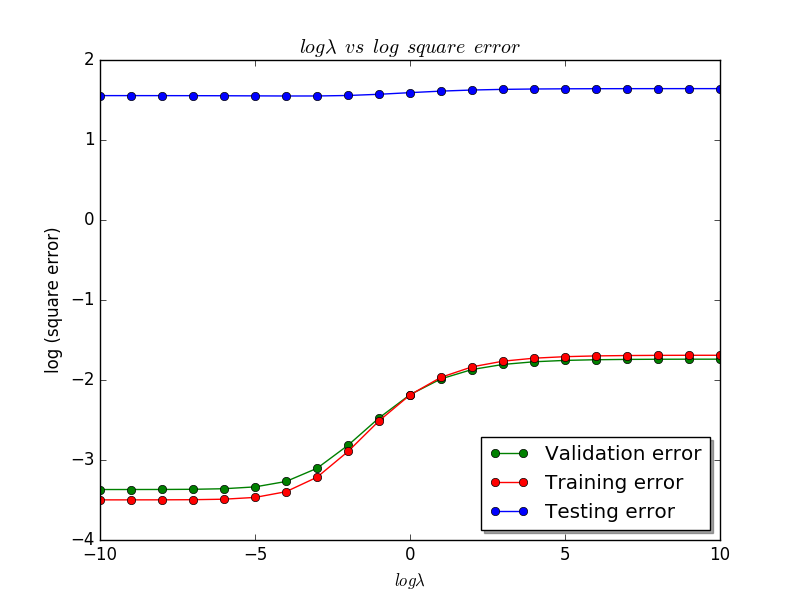
\includegraphics[width=\linewidth]{plot.png}
    \caption{Error Graph}
    \label{fig:Error Graph}
\end{figure}

\section*{Conclusion}

The graph plotted between error and \(\lambda\) gives a clear understanding of variation of error with hyperparameter. The error becomes larger on increasing \(\lambda\). The least error is observed at \({\lambda}\) being \({2^{-10}}\). As \(\lambda\) is decreased, the time taken for executing stochastic gradient descent increases. The error for training data is the least because the \(\omega\) is calculated on this data.


\end{document}

